\chapter[Introduction]{Introduction}
The diversion of significant quantities of \gls{SNM} from the nuclear fuel cycle is a major non-proliferation 
concern \cite{noauthor_serving_2017}. These diversions must be detected in a timely manner using signatures and observables in 
order to properly safeguard the fuel cycle. Timely detection is critical in non-proliferation to discover these shadow fuel cycles
before diverted material is further processed. Pyroprocessing is a used nuclear fuel separations technology for advanced reactors. 
The goal of this research is to identify potential signs of material diversion in a pyroprocessing facility and implement models 
of these processes into a detailed pyroprocessing facility archetype to the modular, agent-based fuel cycle simulator, \Cyclus \cite{huff_fundamental_2016}. This facility archetype will equip users of the \Cyclus fuel cycle simulator to investigate 
detection timeliness enabled by measuring signatures and observables in various fuel cycle scenarios.

\section{Motivation}


\subsection{Future Fuel Cycles}
As the world begins to consider cleaner forms of energy in response to climate change, nuclear energy has regained traction. A main
concern with nuclear power is the pileup of used nuclear fuel (UNF) as a result of the once-through fuel cycle. 
One suggested solution is converting to a closed fuel cycle \cite{wigeland_nuclear_2014}. There are many approaches to transitioning from our current
fuel cycle to a new or closed cycle. Of these future fuel cycles, those involving sodium fast reactors (SFRs) are of interest. 
Pyroprocessing enables a transition from light water reactors (LWRs) to SFRs and other metallic fuel.
Therefore, pyroprocessing is under consideration as a means of processing the fuel required to start up new breeder reactors for
the EG01-EG24 transition scenario.

\subsection{Pyroprocessing}
For other fuel cycle facilities, we have plenty of operating experience to inform safeguards. For example, in the case of aqueous reprocessing
the International Atomic Energy Agency (IAEA) provides detailed flow-sheets of existing facilities \cite{international_atomic_energy_agency_implications_2004}. Multiple modeling
tools have been developed for electrochemical processes such as the Separation and Safeguards Performance Model (SSPM) and Argonne Model for Pyrochemical Recycling (AMPYRE) to combat this lack of operational experience for pyroprocessing plants \cite{maggos_update_2015}. 
These tools take a high fidelity approach to model the
chemistry taking place within each chamber. In order to run these tools, the user must have intimate knowledge of the specific facility the flowsheets have
been designed for. There is a gap, however, in the medium fidelity models that can inform broader fuel cycle applications such as transition scenarios \cite{borrelli_approaches_2017}. 

\subsection{Safeguards}
Currently there are no commercially operated pyroprocessing plants, however various research designs exist in national labs,
notably Argonne National Lab (ANL), Idaho National Lab (INL), and the Korea Atomic Energy Research Institute (KAERI) \cite{michael_f._simpson_developments_2012, lee_advanced, frigo_conceptual_2003}. 
Therefore, prior to construction of any design we 
want to implement safeguards by design. Similar to security by design in next generation reactors, safeguards-by-design incorporates key measurement 
points and access points into the facility design. Rather than learn from mistakes, in the future we aim to incorporate safety 
into the design.

\section{Background}
Prior work has been done on modeling high fidelity facilities and pyroprocessing. In the following section we compile recent efforts modeling fuel cycle facilities, particularly with
\Cyclus. I also breakdown the electrochemical processes of each sub-process in generic pyroprocessing operation. The key elements are voloxidation, electroreduction, electrorefining, and electrowinning. 

\subsection{Facility Modeling}
Developers at the University of Wisconsin and University of Tennessee Knoxville have created a number of detailed facility models to add to the \Cyclus framework. At Wisconsin, Dr. Meghan McGarry contributed various random number generator (RNG) based archetypes to capture non-deterministic behaviors in \texttt{Enrich} and \texttt{Sink} \cite{mcgarry_mbmore_2017}. The capabilities for these archetypes include variable assays, inspector swipe tests, and Gaussian distribution of material. \texttt{CascadeEnrich} adds further detail to the \texttt{Enrich} archetype by incorporating detailed centrifuge physics and parameters. 

\subsection{Pyroprocessing}
Pyroprocessing is an electrochemical separation method used primarily for metallic fast reactor fuel.
This reprocessing technique uses molten salt, whose composition differs depending on the facility.
Molten salt such as LiCl-KCl has a broader stability range compared to water, allowing high potentials to be used for separation.
In aqueous reprocessing, separation would be conducted in a nitric acid and water medium.
This becomes a problem when chemically isolating heavier elements such as lanthanides and actinides.
Controlling the oxidation states of these elements often requires potentials outside the stability of water. 
Increasing a potential beyond the medium's stability (or electrochemical window) limits oxidation and reduction \cite{hayyan_investigating_2013}.
Hence, pyroprocessing was born to improve non-proliferation and reprocessing capabilities.
\\ \\
In addition to the improved redox control of heavier elements, we co-extract materials of interest so they cannot easily be refined for weapons.
This is done through the electrorefining and electrowinning stages by separating a pure uranium stream as well as a uranium/transuranic (U/TRU) mixed stream. 
The U/TRU can then be readily used for fuel fabrication while maintaining proliferation resistance.

Electrochemical separation is the driving force behind pyroprocessing. Electrochemistry relies on the use of Gibbs free energy to determine the required amount of energy to drive a reaction forward.

\begin{figure}[h]
	\centering
	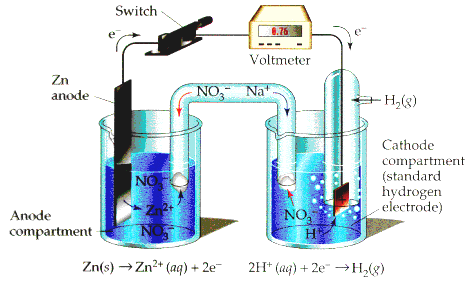
\includegraphics[width=0.8\linewidth]{images/electrochem}
	\caption{Basic example of movement of ions within a galvanic cell, sourced from \cite{angel}.}
	\label{fig:electrochem}
\end{figure}

Figure \ref{fig:electrochem} demonstrates an electrochemical process that generates electricity as a basic example.
The processes described here follow the same principles but require energy to run.
As shown in this basic example, ions are exchanged between the anode and cathode in an attempt to balance the potential difference.
In the case of pyroprocessing, the potential difference is driven by an external source of electricity.
An anode and cathode are used to force the desired ions to deliver charge from one end of the cell to the other.
These ions collect on the surface of the cathode can then be separated from the rest of the solution.
By controlling the voltage of the system as well as the composition of the anode, cathode, and electrolyte we can ensure the removal of unwanted elements/isotopes.


\subsubsection{Voloxidation}
Voloxidation follows the chopping and decladding of the spent fuel. The process is very similar to annealing with regards to materials. The uranium dioxide is heated to temperatures around 700-1000$^\circ C$ which allows gases and some fission products to escape the fuel pellet, as well as convert UO$_2$ to U$_3$O$_8$ \cite{organisation}. Voloxidation, in most cases, takes place in air which provides plenty of oxygen for oxidization of solid UO$_2$, which has the chemical balance \cite{jubin_spent_2009}:

\[ 3UO_2 + O_2 \rightarrow U_3O_8 \]

The above reaction relies on the expansion of uranium at elevated temperatures. A positive feedback is also established: as the uranium dioxide converts to yellowcake powder, the fuel element expands, exposing more uranium dioxide to oxygen. The rate of this reaction/conversion depends on the temperature and gas used. Higher temperatures will yield a faster reaction rate; even ~500 $^\circ C$ is sufficient for 99\% removal in 4 hours.

An added benefit of running a pyroprocessing voloxidation sub-process at the temperatures previously mentioned, 700-1000$^\circ C$, is the removal of gaseous fission products, as shown in Figure \ref{fig:volox}. The
Pyroprocess Integrated inactive Demonstration facility (PRIDE) at KAERI takes it a step further and voloxidates at 1250$^\circ C$ to remove troublesome fission products at the beginning of the cycle\cite{organisation}:

\begin{figure}[h]
	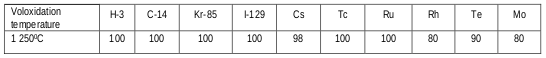
\includegraphics[width=\linewidth]{images/volox_table.png}
	\caption{Voloxidation separation stream composition at 1250 $^\circ C$, units shown are \% mass separated.}
	\label{fig:volox}
\end{figure}

As shown in the table above, pyroprocessing begins with removing a majority of high activity isotopes are removed from the system protecting equipment and personnel. These gases are sent to an off-gas treatment facility that makes use of various scrubbing techniques such as liquid scrubbing, cyrogenic distillation (for removal of Kr), and caustic scrubbing \cite{jubin_spent_2009}.

\subsubsection{Electroreduction}
Following off-gassing and conversion to yellowcake, the non-metallic fuel must be converted and reduced to a molten salt mixture, this is called electrolytic reduction or electroreduction.
In most cases this is done with a LiCl-KCl salt eutectic combined with a Li$_2$O catalyst. The electrolytic reduction phase consists of three main parts: UO$_2$ recovery, reduction, and rare earth (RE) removal.

\begin{figure}[h]
	\centering
	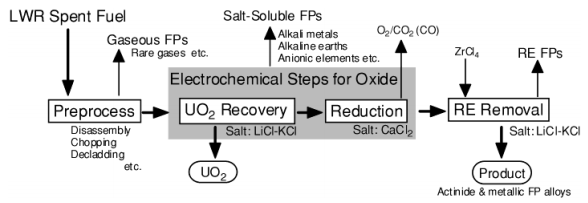
\includegraphics[width=\linewidth]{images/reduction_flow}
	\caption{Electroreduction flow sheet \cite{ohta}.}
\end{figure}

The chemical balance for an anode and cathode in a LiCl-KCl salt is as follows:

\[ UO_2 \rightarrow UO_2^{2+}(LiCl-KCl) + 2e^{2-} \hspace{6mm} anode \]
\[ UO^{2+}(LiCl-KCl) + 2e^{2-} \rightarrow UO_2 \hspace{6mm} cathode \]

As in other separations technologies, noble metals can often follow the uranium through the rest of the process.
The lurking noble metal fission products (FPs) cause an increase in radioactivity of the UO$_2$ stream. 
Therefore, the weight percent dissolution of uranium is critical in reducing the amount of noble metal FPs that follows to the product stream.
Lithium oxide can also be used as a catalyst to draw uranium to the cathode while leaving the noble metal fission products in the salt.
This is done with 1-3wt\% Li$_2$O in the following equations \cite{hur_electrochemical_nodate}:

\[ Li_2O \rightarrow 2Li^+ + O^{2-} \]
\[ UO_{x/2} + xLi \rightarrow U + xLi_2O \]

These equations make a continuously driven loop dragging uranium (either UO$_2$ or U$_3$O$_8$) from the anode to the cathode. 
Disassociated lithium ions from the first equation break apart the uranium and oxide, with help from the electric potential.
The uranium collects on the cathode while the Li$_2$O is recycled and drives the first equation forward again. 
Reduction then occurs on the cathode where the U, TRU, rare earths, and noble metals (NMs) have collected.
This is achieved by evolving oxygen gas along the anode using the following reactions\cite{hur_electrochemical_nodate,organisation}:

\[ Li^+ \rightarrow Li + e^- \hspace{10mm} Cathode \]
\[ M_xO_y + 2yLi \rightarrow xM + yLi_2O \hspace{10mm} Cathode \]
\[ O^{2-} \rightarrow 0.5O_2 + 2e^- \hspace{10mm} Anode \]

Electrochemical reduction results in an alloy of reduced uranium, transuranics, rare earths, and noble metals; however, we want to minimize the amount of rare earths and noble metals in the product.
The RE FPs can be removed from the alloy by substituting another chloride into the LiCl-KCl eutectic.
Ohta et al. explored the use of ZrCl$_4$ as this substitue which changes the chemical balance to the following \cite{ohta}:

\[ 3ZrCl_4(LiCl-KCl) + RE \rightarrow 3Zr + 4RECl_3(LiCl-KCl) \]

Yakamura demonstrates this process to have a decontamination factor of 10 with regard to separating REs from actinides \cite{sakamura}. Additionally, by using Zr as the metal substitute, it is compatible with fuel fabrication later \cite{ohta}.
\subsubsection{Electrorefining}
Electrorefining is the primary process in pyroprocessing, and is the first stage for fast reactor fuel, since metallic fuel does not require reduction or chopping.
In addition to being the most important process, it is also the most complex with a multitude of input parameters and material streams. 
The goal of the refining process is to separate the uranium and TRU from the alloy ingot formed in the reduction phase.
Two streams will be formed for the fabrication of fuel: one stream that is a mix of U/TRU at the desired ratio, and the other a pure stream of uranium.
The refining efficiency relies on temperature and current primarily, however, advanced methods are being developed.
KAERI, for example, has investigated adding a central stirrer, lowering pressure, and rotating the anode \cite{lee_advanced}.
The rotation aims to mix the uranium in the salt such that none gets stuck on the bottom or edges of the vessel. 
Stirring too vigorously, however, can lead to the removal of uranium dendrites from the cathode thereby decreasing efficiency.\\

The governing reactions that allow this process to work are based on the stability constants and oxidation potential of the remaining FPs.
The voltage used,  0.5-1V, is such that uranium is unstable in the chloride form \cite{organisation}, while TRUs have a higher stability. 
This leads to TRU remaining in chloride form, along with some uranium, and pure uranium accumulating on the cathode.
The chloride reaction follows the below equation, and will run to the right as long as there is uranium within the salt \cite{organisation}.

\[ UCl_3+TRU(RE) \rightarrow U + TRU(RE)Cl_3 \]
\[ UCl_3 + 3Na \rightarrow 3NaCl + U \]
\[ UCl_3 + 3Cs \rightarrow 3CsCl + U \]
\[ UCl_3 + Pu \rightarrow PuCl_3 + U \hspace{10mm} \delta G = -22.44kcal \]
\[ 4UCl_3 + 3Zr \rightarrow 3ZrCl_4 + 5U \hspace{10mm} \delta G = 31.123kcal \]

As shown by the reactions above, the TRU have a negative Gibbs free energy value for spontaneous reactions while the transition metals do not \cite{supy}.
This leads to the transition metals remaining in the anode basket while the TRU are drawn into the liquid cadmium cathode \cite{lee_korean_2011}.


\subsubsection{Electrowinning}
The electrorefiner accumulates TRUs and rare earth fission products within the salt.
These isotopes build up and require separation and disposal, therefore the salt from the refiner is sent to the electrowinner.
This stage further purifies the salt by targeting the electric potential of TRUs, RE, and U again \cite{lee_korean_2011,organisation}.
Placed in liquid cadmium once again, the three groups have overlapping electric potentials leading them all to deposit in the cadmium \cite{lee_korean_2011}. 
While the refiner's role is to generate a stream of pure uranium, the electrowinner performs co-extraction of uranium and TRUs.
This inherent proliferation resistance is a main draw of the pyroprocessing technique.
Rare earths are still present on the cadmium and further separations must be conducted.
These elements are removed through the addition of CdCl$_2$ which oxidizes the rare earths, while the uranium and TRUs are unaffected.
These oxidized elements fall back into the salt, leaving the purified U/TRU stream on the electrowinner.


Although the facility is great in terms of safeguards, pyroprocessing has its share of drawbacks as well.
Currently, pyroprocessing can only be performed as a batch process, which significantly limits throughput compared to a continuous facility. 
Additionally, the safety and economic concerns of running a molten salt plant are much greater than a nitric acid one.
Despite these downsides, pyroprocessing is an efficient use of electrochemical separation and a leader in proliferation resistant separations.

ANL, INL, and KAERI, among other entities, have produced pyroprocessing facility designs.
In order to encompass a broad range of flowsheets, we must take a generic approach when modeling pyroprocessing. Accordingly, this work includes the following sub-processes: voloxidation, electroreduction, electrorefining, and electrowinning. 
While electrorefining is the process of primary concern, each of the processes has an important role. 

\section{Goals}

This work aims to generically model a pyroprocessing facility with medium fidelity, appropriate for simulating diversion scenarios. Modeling
this within \Cyclus enables us to explore the capability of modeling sub-facilities and diversion. In addition, we use this higher fidelity model to verify transition
scenarios such as EG01-EG24 within \Cyclus \cite{wigeland_nuclear_2014}. Finally we aim to identify impactful facility parameters for
various facility layouts through sensitivity analysis. 